\documentclass[a4paper,11pt]{article}

\usepackage[plain]{fullpage} %Error.
\usepackage{graphicx}  %This enables the inclusion of pdf graphic files in figures
\usepackage{wrapfig}
\usepackage{array}
\usepackage[hidelinks]{hyperref}
\usepackage{color}
\definecolor{light-gray}{gray}{0.95}
\usepackage{listings}
\lstset{
basicstyle=\scriptsize, 
morecomment=[l]{/*},
backgroundcolor=\color{light-gray}, 
xleftmargin=.10in,
xrightmargin=.10in,
language=C
}

\title{\textbf{Report: Assignment 3}}
\author{Group 9: \O yvin Richardsen, Sandor Zeestraten, Stian Habbestad}
\date{{Norwegian University of Science and Technology \\
TDT4258 Energy Efficient Computer Design \\}
\today}
 
\begin{document}
\maketitle

\begin{abstract}


In this assignment we write C code for an AVR microcontroller on linux. Through this assignment we aim to become more familiar with C coding for AVR32, linux and how to write a driver for linux. Our approach was to first replicate the features of the previous assignment, then we ..................
\end{abstract}

\bigskip
\tableofcontents
\newpage

\section{Introduction}

In this exercise we write a game in C, which is executed on top of linux on a STK1000 development board. We have written a pair of drivers to handle leds and buttons...................

\section{Description and methodology}

\textbf{Forrige rapport: organize report better (overview and block diagram before description of code fragments and functions). Ergo, block diagram her?}\\

First off we started out with trying to install linux on the STK1000 development board. This turned out to be a tricky affair. We had a step by step guide for compiling linux that we followed, but with no luck. Luckily there was mentioned an image of a precompiled linux that we could extract to the SD card. After some mixing back and forth with environment variables from the other u-boot.bin file(from itslearning) into the one we were using we finally started to get somewhere. 

\textbf{(d e bare å korrigera osv) }

Once we had linux up and running we started out with a simple "Hello world" program to verify things were working. Now we started out with programming a driver for the LEDs. We sometimes thought we had found the solution, but we still hadn't figured it out correctly. We gave the LED driver a pause and started to communicate with the frame buffer in linux. 

First off we thought maybe this file had to be a kernel module as well, but we soon understood that we needed acceess to quite a few libraries to make the memory mapping work. We started with generating a random bit values for the display and went on with more logical values, for example a third of the screen was made red. As we tried to read bit values from an image of the file format bitmap, we started to see that there were some errors in regards to how we read the file. 

From a previous course we had implemented sokoban in Java, so we figured this game would fit neatly for this exercise, thus we translated it into C. 

\emph{linux compiling, image to sd, previous assignment, driver(led and button), framebuffer, porting of sokoban to C, sound, generated sounds, }



%We started out by implementing the previous assignment that we had coded in assembly, only this time in C. This was an easy start for implementing an interrupt routine in C based on a program we had already designed. The primary challenge was making the buttons work with interrupts. Once we had a functional program with buttons and LEDs, we were ready to start working on the ABDAC. We started by simply trying to enable the ABDAC while still retaining the rest of the functionality. This proved troublesome at first, because interrupts from the buttons stopped working as soon as we enabled interrupts from the ABDAC. We decided to work around this by having the buttons and the ABDAC connected to different PIOs, which solved our problem. The next step was generating random noise and sending samples to the ABDAC. This proved to be rather trivial, we simply wrote the first sample to the ABDAC from the button interrupt routine, and then used interrupts from the ABDAC to retrieve the next sample (random in this case) and write it to the ABDAC.




\begin{lstlisting}
void abdac_isr(void) {
	(...)
	/* Send sample to ABDAC */
	dac->SDR.channel0 = (short) *current_wave_ptr;
	dac->SDR.channel1 = (short) *current_wave_ptr;
	sample_counter++;
	current_wave_ptr++;
}
\end{lstlisting}

%Then we started working on the specific sounds we wanted our program to play. We wrote a function for mathematical generation of sine wave samples, and created sample vectors based on frequency levels of musical tones. 

\begin{lstlisting}
/* Generate the sample vector for ~one period of a pure sine wave */
void generateSine(float f) {
	set_sample_size(f);
	int i;
	for (i = 0; i < sample_size; i++) {
		*current_wave_ptr = (int) floor(A*sin(f*(2*M_PI)*i/Fs));
		current_wave_ptr++;
	}
\end{lstlisting}

%We then added sample vectors together to create longer sounds, and tested this by writing samples to the ABDAC in the same way as with random noise.
\begin{lstlisting}
void button_isr(void) {
	(...)
	if (buttons == BUTTON7) {
		current_sound_ptr = test_sound;
		current_sound_tl_ptr = test_sound_tone_length;
		sound_length = test_sound_length;
		LED_VECTOR = LED7;
	}
	(...)
	init_sound(); // Start playing the sound
	(...)
}
/* Initialize sound counters and pointers, and send first sample to ABDAC */
void init_sound(void) {
	(...)
	set_tone(*current_sound_ptr);
	set_tone_length(*current_sound_ptr, *current_sound_tl_ptr);
	dac->SDR.channel0 = (short) *current_wave_ptr;
	dac->SDR.channel1 = (short) *current_wave_ptr;	
	(...)
}
\end{lstlisting}

%Through this we were able to play simple musical melodies. Because of our choice to play musical tones (up to a frequency of 2093Hz), we used the undivided clock frequency of OSC1 for the ABDAC in order to get the best possible sound quality (attempts to use the divided frequency screwed up our sounds). This meant the sampling frequency \textit{Fs} for our program would be 12MHz/256 ~ 47KHz. We also experimented with generating sawtooth, square, triangle and frequency modulated waves (also mathematically) to increase the diversity of our possible sounds, but ended up with only implementing the triangle waves in addition to pure sine. Finally we added tones with appropriate lengths together to make the microcontroller play the well known melody of "Tetris". 

\begin{lstlisting}
/* Frequency levels for various tones */
#define C6 1046.50f
#define D6 1174.66f
#define E6 1318.51f

/* Tone sample arrays */
#define default_sample_size 100
volatile int C6_wave[default_sample_size];
volatile int D6_wave[default_sample_size];
volatile int E6_wave[default_sample_size];

/* Tone lengths (seconds) */
#define E 0.125			// 1/8
#define Q 0.25			// 1/4

float tetris[] = { E6, B5, C6, D6, C6, B5, A5, A5, C6, E6, D6, C6, B5, (...) };
float tetris_tone_length[] = { Q, E, E, Q, E, E, Q, E, E, Q, E, E, Q,  (...) };
int tetris_length = sizeof(tetris)/sizeof(*(tetris));
\end{lstlisting}

%As an extra touch, we spent some time trying to get rid of the random noise we ended up with after playing our sounds. By tweaking the debounce delay properly and resetting the ABDAC after the final sample was played, all unwanted noise disappeared. See Figure 1 below for a full state diagram of how the program works.

\begin{center}
\centering
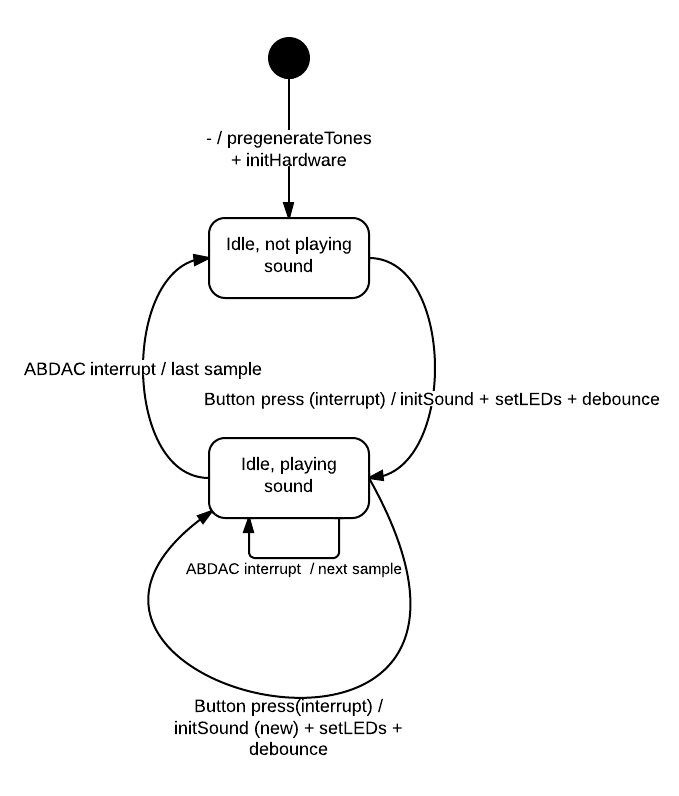
\includegraphics[scale=0.75]{images/lucid_chart.png}
\linebreak
Figure 1: State Diagram of the program
\end{center}

\newpage

\subsection*{Debugging}

%Here is a screenshot (Figure 2) showing us debugging our \emph{generateTriangle} function which generates triangle sound wave samples. More specifically we check that the values we get from each part of our (complex) mathematical expression are valid. 

\begin{center}

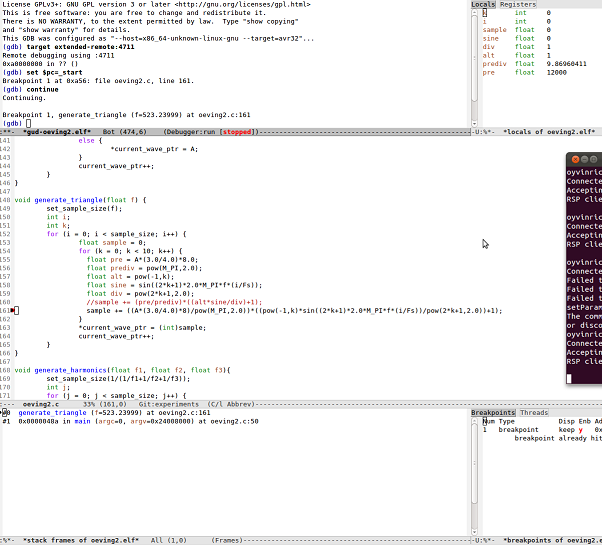
\includegraphics{images/debugsmall.png}
Figure 2: Debugging the \emph{generateTriangle} function
\end{center}

\section{Results}
%The result of the exercise is that we coded a single program in C which generates and plays four different sounds when different switches (\emph{SW7} to \emph{SW4}) are pressed. At the start of the program it generates tones (\emph{A4} to \emph{C7}) based on the sine and triangle waves. Then once it gets an interrupt from a switch it plays the first sample of that switch whereafter the ABDAC generates an interrupt which plays the next sample until it is finished.

\section{Tests}
\paragraph{Description}
%We've created a few test scenarios in order to test different cases of our code for playing sounds. The tests were conducted by a person interacting with the switches wearing a headset, and another person logging the results. The main equipment was the STK1000 development board, JTAGICE MKII and a headset. The jumpers of the board were set as specified in the compendium (section 3.4.1) \cite{komp}. The GPIO was connected as following: Port B to the LEDs and Port C to the switches.

\paragraph{Results}
%Below is a table of the different tests we ran, the preconditions and the results. We did not pass the \emph{Bouncing} test. Here we checked whether a sound would play without any interruptions during a switch press (both up and down). Releasing the button provides a new interrupt, which calls the button interrupt routine of our program, which further delays the waiting sound sample, causing a noticeable effect on the sound.

\begin{center}
\footnotesize
\renewcommand{\arraystretch}{1.25} %vertical cell padding
\begin{tabular}[pos]{|m{45pt}|m{80pt}|m{90pt}|m{105pt}|m{60pt}|}
\hline  \textbf{Name} & \textbf{Description} & \textbf{Conditions} & \textbf{Expected} & \textbf{Results} \\ 

\hline Steady-state test & Power is on and the main program is running & The board has been programmed and powered on & The board is powered and no LEDs or sounds should be on & Passed \\

\hline SFX1 & The first SFX plays & The main program is running & \emph{SFX1} plays once after \emph{SW7} is pressed. \emph{LED7} should be turned on & Passed \\

\hline SFX2 & The first SFX plays & The main program is running & \emph{SFX2} plays once after \emph{SW6} is pressed. \emph{LED6} should be turned on & Passed \\

\hline SFX3 & The first SFX plays & The main program is running & \emph{SFX3} plays once after \emph{SW5} is pressed. \emph{LED5} should be turned on & Passed \\ 

\hline Intro theme & The intro theme plays & The main program is running & The intro theme plays once after \emph{SW4} is pressed. \emph{LED4} should be turned on & Passed \\

\hline Bouncing & Any sound should only be played once per press of switch & Press down any switch from \emph{SW7} to \emph{SW4} and let it go & The sound should finish playing without any interruptions & Failed \\

\hline Change sound & Play a sound while another sound is already playing & A switch has been pressed and a sound is playing. While playing another switch has been pressed & The sound of the newly pressed switched should be playing & Passed \\ 

\hline Stop & Stop playing sounds when pressing any switch from \emph{SW3} to \emph{SW0} & Press any switch from \emph{SW3} to \emph{SW0} while sound is playing & The sound should stop playing & Passed \\ 

\hline 
\end{tabular} 
\end{center}

\newpage

\section{Evaluation of assignment}
%This assignment was more demanding yet also more fun than the first assignment. The learning curve was a bit harder as not all of us had coded much in C before, but it was a nice opportunity to learn.

\section{Conclusion}
%We learned how to generate and play different sounds in C. This will be helpful when we start coding the next assignment. In the end we have four different sounds. Three short sound effects and one melody. 

\footnotesize{  % This makes the Reference items print in footnotesize fonts
\begin{thebibliography}{N}

\bibitem[1]{avrdoc} AVR32 Architecture Document
\url{http://www.atmel.com/images/doc32000.pdf}

\bibitem[2]{stkdoc} AT32AP7000 Datasheet
\url{http://www.atmel.com/Images/doc32003.pdf}

\bibitem[3]{komp} TDT4258 Compendium
\url{http://www.idi.ntnu.no/emner/tdt4258/_media/kompendium.pdf}

\end{thebibliography}  
}

\end{document} 
